\documentclass[conference]{IEEEtran}
\IEEEoverridecommandlockouts

\usepackage{cite}
\usepackage{amsmath,amssymb,amsfonts}
\usepackage{algorithmic}
\usepackage{graphicx}
\usepackage{textcomp}
\usepackage{xcolor}
\def\BibTeX{{\rm B\kern-.05em{\sc i\kern-.025em b}\kern-.08em
    T\kern-.1667em\lower.7ex\hbox{E}\kern-.125emX}}
\begin{document}

\title{Plant disease identification in leaf images using multi-scale high-resolution  visual transformers with linear projection for feature reduction}

\author{\IEEEauthorblockN{Rakhat Yskak}
\IEEEauthorblockA{\textit{School of Engineering and Digital Sciences} \\
\textit{Nazarbayev University}\\
Astana, Kazakhstan}}

\maketitle
\begin{abstract}
For this project, I used Vision Transformers and High-Resolution Networks to create a framework for automatically identifying plant diseases. The model achieved a micro-averaged F1-score of 0.98 and a Hamming loss of 0.025 after being trained on a customised subset of the PlantVillage dataset and assessed using micro and macro-averaged metrics. The outcomes demonstrate the efficacy of the model and its potential for use in agriculture.
\end{abstract}

\section{Introduction}
Reducing agricultural losses and guaranteeing food security depend on the precise and timely detection of plant diseases. Conventional disease detection techniques frequently depend on labour-intensive, human-error-prone manual checks. While deep learning methods, especially convolutional neural networks (CNNs), have made image-based illness identification better, they have trouble capturing both high-resolution details and global characteristics at the same time.

In order to overcome these constraints, I suggest a method that combines High-Resolution Networks (HRNet) with Vision Transformers (ViTs) for the effective and precise classification of plant diseases. In order to improve classification performance, this method makes use of HRNet for multi-scale feature representation and ViTs for global feature extraction.

\section{Methodology}
\subsection{Model Architecture}
My project's central component is a model that efficiently captures and processes high-resolution information by fusing the ideas of ViT and HRNets. Recent methods from \cite{wang2020} and \cite{gu2021} are used in this design.

First, each input image $x \in \mathbb{R}^{H \times W \times C}$ is divided into non-overlapping $N$ patches of size $p \times p$:
\begin{equation}
    N = \frac{H \cdot W}{p^2}
\end{equation}
Then, to each embedded patch we add their positional embeddings:
\begin{equation}
    z = E \cdot x_{\text{patch}} + P
\end{equation}
where $E$ is the patch embedding matrix and $P$ denotes the positional embeddings. This ensures that the model preserves the spatial structure\cite{sebastian2024}.

My inspiration to combine HRNet with ViT, came from the architecture of multi-scale high-resolution ViTs by \cite{gu2021}, which gradually grows to four branches and contains several modules with multiple Transformer blocks in each step.

\begin{figure}
    \centering
    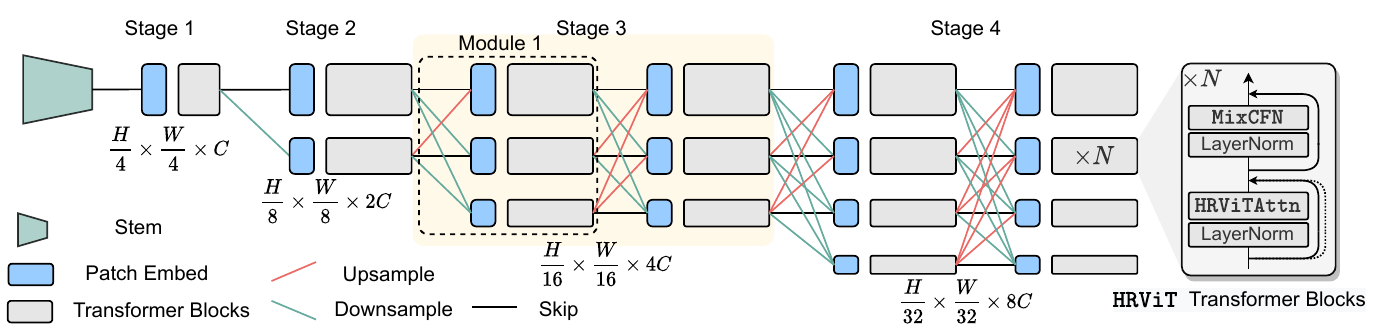
\includegraphics[width=\linewidth]{hrvit.png}
    \caption{The overall architecture of HRViT.}
    \label{fig:enter-label}
\end{figure}

The fusion mechanism across multiple resolutions is defined as:
\begin{equation}
    x^l_i = \sum_{j=1}^s F_{ij}(x^{l-1}_j)
\end{equation}
$x^l_i$ represents the feature map at resolution $i$ in layer $l$, $s$ is the number of resolutions, and $F_{ij}$ is the transformation function, combining convolutional and attention operations for effective feature fusion.

\subsection{Dataset and Preprocessing}
Since ViTaL's dataset is unavailable online, I decided to use a similar one with the same classes but different images \cite{sebastian2024} for a fair comparison between models. Therefore, my dataset contains 11 classes with 275 images per class to ensure class balance. 

I applied a series of preprocessing and augmentation techniques to enhance the model's performance, including:

\begin{enumerate}
    \item Resizing with bilinear interpolation.
    \item Min-max normalization:
    \begin{equation}
        x_{\text{norm}} = \frac{x - \mu}{\sigma}
    \end{equation}
    where $\mu = [0.485, 0.456, 0.406]$ and $\sigma = [0.229, 0.224, 0.225]$ \cite{Dosovitskiy2020}.
\end{enumerate}

\subsection{Data Augmentation}
To reduce overfitting and improve the model's generalization capabilities, I applied the following augmentations:
\begin{enumerate}
    \item Random horizontal flip with a probability of $0.5$ to introduce variability.
    \item Random rotation from $[-15^\circ, 15^\circ]$ to account for different orientations.
    \item Color jitter to simulate varying lighting conditions.
\end{enumerate}
These augmentations were essential in ensuring the model performed well under different conditions, as highlighted in related work \cite{sebastian2024}.

\subsection{Training}
Model was trained using the cross-entropy loss function and the AdamW optimizer over 50 epochs with a batch size of 32, a learning rate of $1 \times 10^{-4}$, and a weight decay of $1 \times 10^{-5}$. Moreover, implemented early stopping if the validation loss did not improve over 10 consecutive epochs \cite{sebastian2024}.

\section{Results}

The model's performance was evaluated using micro and macro-averaged precision, recall, and F1-score, along with the Hamming loss as in \cite{sebastian2024}. The results are summarized in Table \ref{tab:metrics}.

\begin{table}[h]
\centering
\caption{Performance Metrics}
\label{tab:metrics}
\begin{tabular}{|l|c|c|}
\hline
Metric & Micro Average & Macro Average \\ \hline
Precision & 0.98 & 0.975 \\ \hline
Recall & 0.98 & 0.975 \\ \hline
F1-Score & 0.98 & 0.975 \\ \hline
Hamming Loss & \multicolumn{2}{c|}{0.025} \\ \hline
\end{tabular}
\end{table}

The Hamming Loss of $0.025$ indicates a low rate of incorrect predictions, demonstrating the model's strong performance across all classes.

The confusion matrix in Figure \ref{fig:confusion_matrix} shows only a few misclassifications, primarily in visually similar classes.

\begin{figure}[h]
\centering
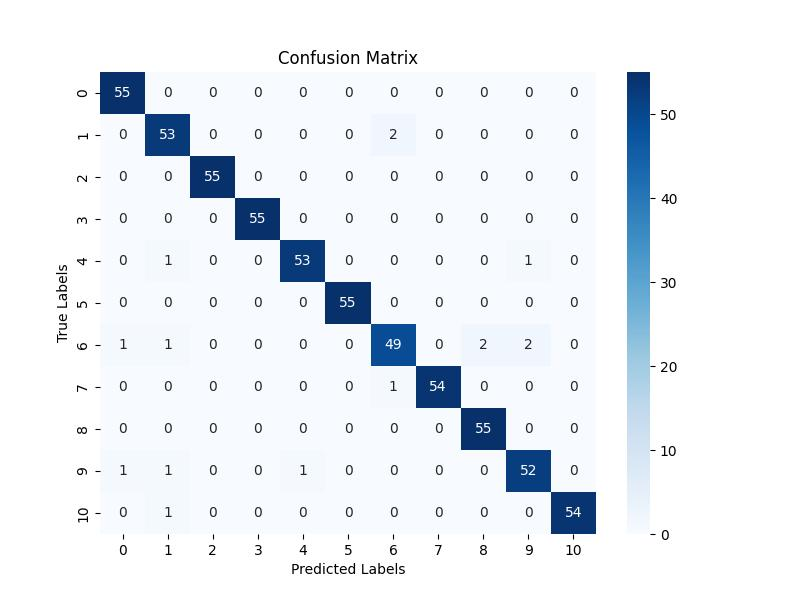
\includegraphics[width=1\linewidth]{confusion_matrix.jpg}
\caption{Confusion Matrix}
\label{fig:confusion_matrix}
\end{figure}

The training and validation loss curves in Figure \ref{fig:loss_curves} show a steady decrease, indicating good generalization despite the small dataset.

\begin{figure}[h]
\centering
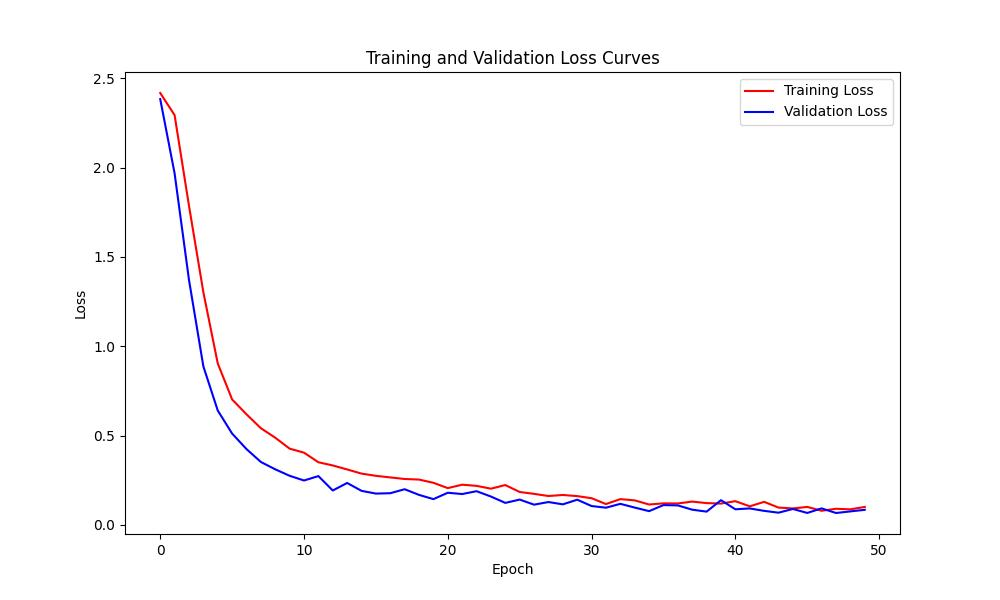
\includegraphics[width=1\linewidth]{loss_curves.jpg}
\caption{Training and Validation Loss Curves}
\label{fig:loss_curves}
\end{figure}

\section{Discussion}
Proposed model demonstrates high precision, recall, and F1-scores, with an overall strong performance. Despite the small dataset size, the model generalizes well, as evidenced by the consistent training and validation loss curves. However, minor misclassifications in similar disease classes suggest that a larger and more diverse dataset could further improve performance. Future work could explore additional augmentation techniques to enhance class separation.

\section{Conclusion}
In this project, I developed the model for automated plant disease identification using Vision Transformers and High-Resolution Networks. The model demonstrated strong performance, suggesting its potential for practical agricultural applications. Future improvements could include training on a larger, more diverse dataset to enhance model robustness.


\bibliographystyle{ieeetr}
\bibliography{ref}

\end{document}
